\chapter{SKOS---managing vocabularies with RDFS-Plus}
\label{ch11}



\section{Simple Knowledge Organization System (SKOS)}
\label{ch11.skos}
SKOS (the Simple Knowledge Organization System) is a W3C Recommendation
that provides a means for representing knowledge organization systems
(including controlled vocabularies, thesauri, taxonomies, and
folksonomies) in a distributed and linkable way. Knowledge Organization
Systems have been around for a long time, most formally as part of
Library Science, but means for representing and exchanging them in a
computer network have not.

Given the existence of several thesaurus standards, one could well
wonder why people found it necessary to create another one. The key
differentiator between SKOS and existing thesaurus standards is its
basis in the Semantic Web. Unlike existing standards, SKOS was designed
from the start to allow modelers to create modular knowledge
organizations that can be reused and referenced across the Web. SKOS was
not designed to replace any thesaurus standard but in fact to augment
them by bringing the distributed nature of the Semantic Web to thesauri
and controlled vocabularies. Toward this end, it was also a design goal
of SKOS that it be possible to map any thesaurus standards to SKOS in a
fairly straightforward way.

SKOS satisfies the goals of distributing and linking vocabularies by leveraging
all of the features of RDF, RDFS and linked data that we have seen so far in this book. 
By using RDF as its basis, SKOS allows vocabularies to link not only to other vocabularies, but 
indeed to any data set (or metadata set) represented in RDF, including 
models represented in RDFS, RDFS-Plus and OWL. 

As an example of using SKOS, for many years, the United Nations Food and
Agriculture Organization has maintained a thesaurus called AGROVOC for
organizing documents about agriculture. Figure~\ref{fig:ch11.1} shows a sample from
the SKOS publication of AGROVOC. The diagram shows six concepts, which
are related to one another by various properties that are defined in the
SKOS Core. Data properties are shown within the boxes corresponding to
the concepts. As we shall see, each of these properties is defined in
relation to other properties, so certain useful inferences can be made.

\begin{figure}
\centering
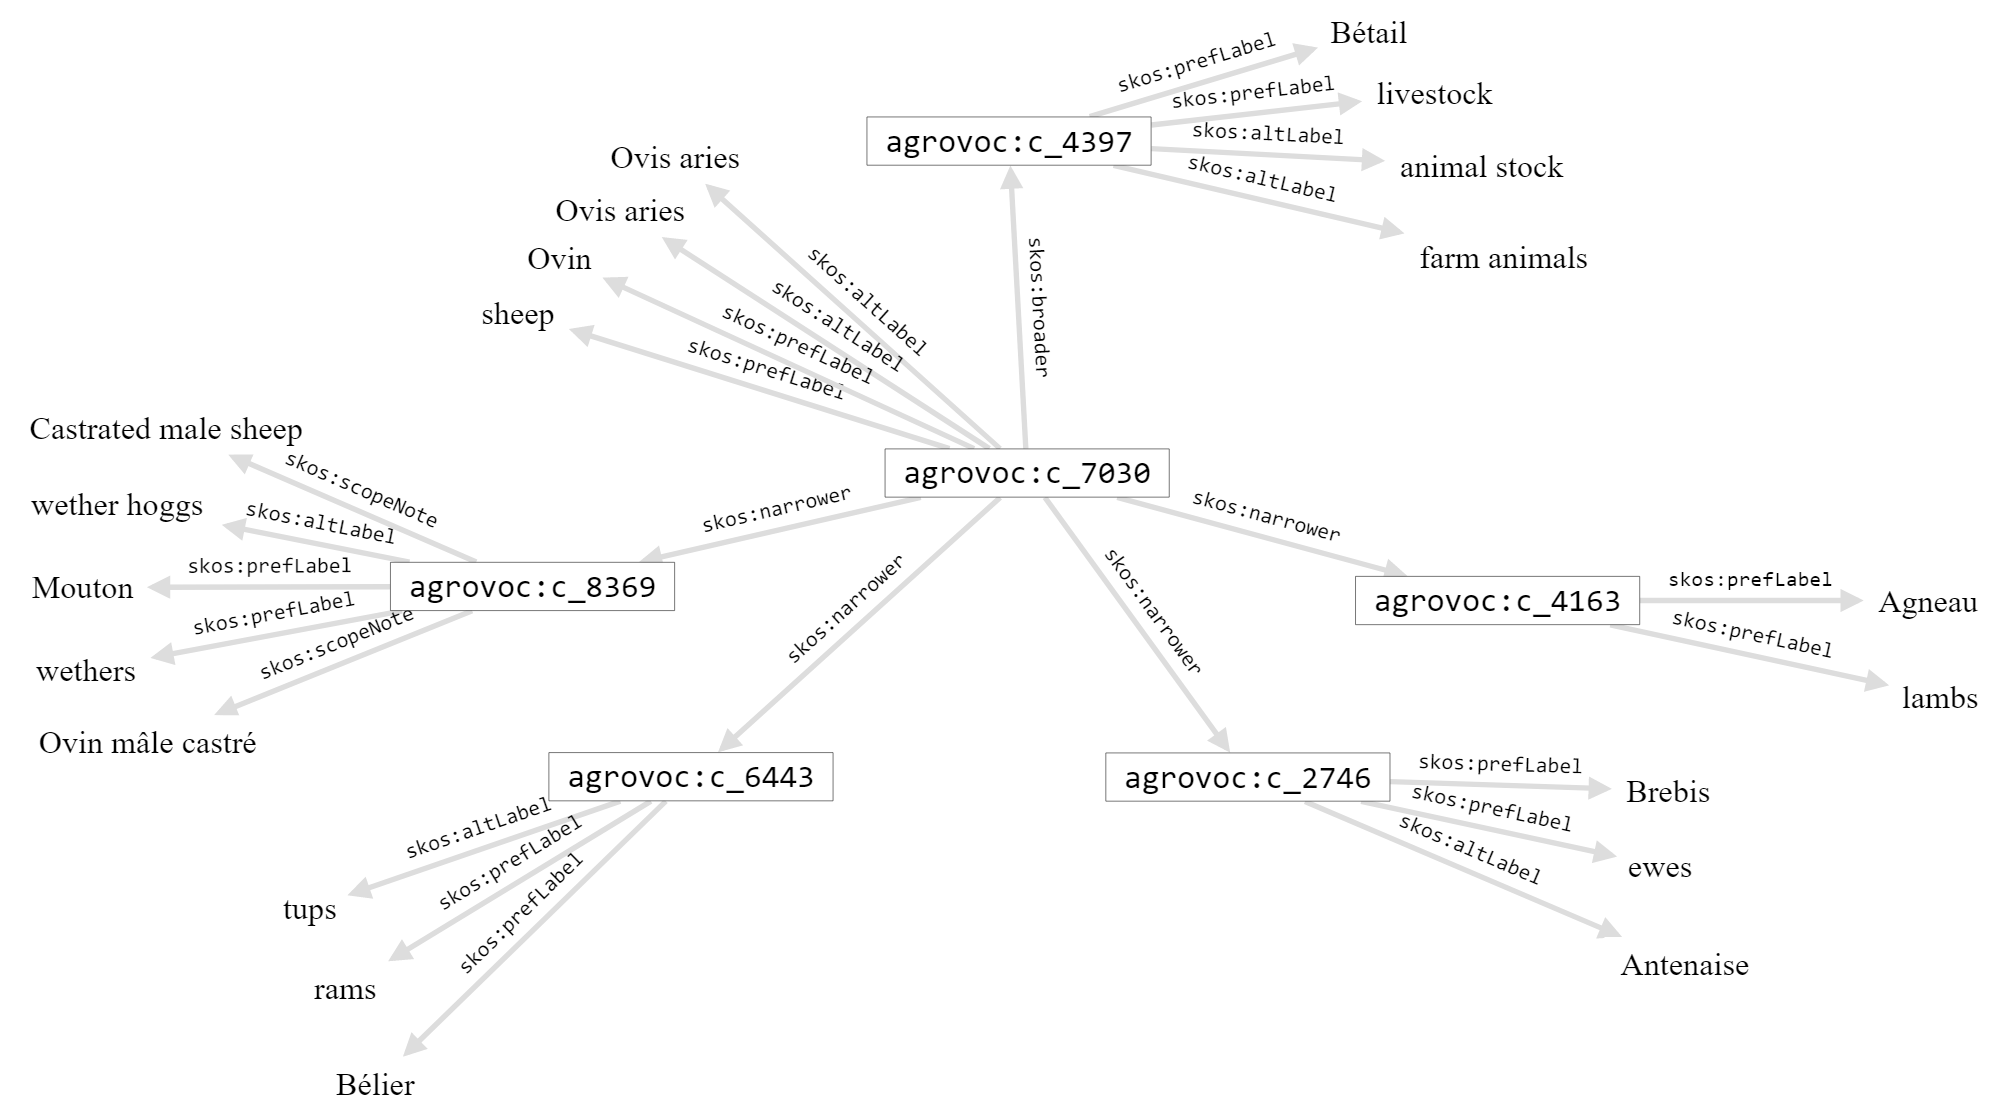
\includegraphics[width=5in]{SWWOv3/media/ch11/figure11-1.png}
\caption{Sample concepts from AGROVOC.}
\label{fig:ch11.1}
\end{figure}


The same information from Figure~\ref{fig:ch11.1} is shown as triples in Turtle
here:

\begin{lstlisting}
agrovoc:c_4397
  a skos:Concept ;
  skos:prefLabel "B(*@\'e@*)tail"@fr , "Livestock"@en ;
  skos:altLabel "Animal stock"@en , "Farm animals"@en .
agrovoc:c_2746
  a skos:Concept ;
  skos:prefLabel "Brebis"@fr , "Ewes"@en ;
  skos:altLabel "Gimmers"@en , "Antenaise"@fr , "Ewe hoggs"@en .
agrovoc:c_4163
  a skos:Concept ;
  skos:prefLabel "Agneau"@fr , "Lambs"@en .
agrovoc:c_6443
  a skos:Concept ;
  skos:prefLabel "B(*@\'e@*)lier"@fr , "Rams"@en ;
  skos:altLabel "Tups"@en .
agrovoc:c_8369
  a skos:Concept ;
  skos:prefLabel "Wethers"@en , "Mouton"@fr ;
  skos:altLabel "Wether hoggs"@en , "Hoggets"@en ;
  skos:scopeNote "Ovin m(*@\^a@*)le castr(*@\'e@*)"@fr , "Castrated male sheep"@en .
agrovoc:c_7030
  a skos:Concept ;
  skos:prefLabel "Sheep"@en , "Ovin"@fr ;
  skos:altLabel "Ovis aries"@en , "Ovis aries"@fr ;
  skos:broader agrovoc:c_4397 ;
  skos:narrower agrovoc:c_2746, agrovoc:c_6443, agrovoc:c_8369,
                agrovoc:c_4163 .
\end{lstlisting}

First, let's look at the \textit{Concepts} in SKOS. This excerpt defines six of them, and specifies
names for them.  But what is a "Concept", and how does it relate to things we already know about, 
like Classes?  The main motivation for SKOS comes from Library Science, where we want to have ways to describe our 
published works.  A Concept in SKOS is one way to do that.  Unlike Classes in RDFS, Concepts in SKOS have no formal correspondence in mathematics. A Concept in SKOS is a simply a categorization for published works; as such, the terms defined in SKOS don't have as strict a formal definition as the terms defined in RDFS and OWL.  As we will see later in this chapter, SKOS makes use of the formal structures in RDFS-Plus to describe how Concepts work and how they can be related to one another. 

Second, let's look at internationalization. SKOS is maintained by the UN
in several languages, including English and French; each concept has
labels in multiple languages. None of these languages can take
precedence over any other---so the UN uses numbers instead of names as
the basis of the URI's for resources in AGROVOC. The human readable
names are given as strings associated with the concepts in a variety of
ways. Strings in Turtle optionally include a language tag (taken from
the XML standard) to indicate the language they are written in---in this
fragment, we have retained labels in English (``en'') and French
(``fr'').

Next, let's look more closely at those strings, and how labels are
managed in SKOS. As we have seen before, there is already a label
resource defined in RDFS: rdfs:label. Although rdfs:label has no formal
semantics defined (that is, there are no inferences that concern
rdfs:label), it does have the informal meaning that it is something that
can be used as the printable or human readable name of a resource. SKOS
provides a more detailed notion of a concept's label, in accordance with
usual thesaurus practice. In particular, it defines three different
kinds of labels: a preferred label, an alternative label, and a hidden
label. These are defined in SKOS with the following triples:

\begin{lstlisting}
skos:prefLabel
  a rdf:Property ;
  rdfs:label "preferred label"@en ;
  rdfs:subPropertyOf rdfs:label .
skos:altLabel
  a rdf:Property ;
  rdfs:label "alternative label"@en ;
  rdfs:subPropertyOf rdfs:label.
skos:hiddenLabel
  a rdf:Property ;
  rdfs:label "hidden label"@en ;
  rdfs:subPropertyOf rdfs:label .
\end{lstlisting}

The SKOS definition includes a number of other triples defining these
properties, but we will concentrate on these for this description.

Notice that each property has an \texttt{rdfs:label}, which provides a human
readable version of the name of each resource. Furthermore, each of
these properties is declared to be of type \texttt{rdf:Property}. Finally, each
of these is declared to be a subproperty of \texttt{rdfs:label}. What does this
mean in terms of RDFS-Plus?

As we have already seen, \texttt{rdfs:subPropertyOf} propagates triples from the
subproperty to the superproperty. In the first case, from any triple
using \texttt{skos:prefLabel} as a predicate, we can infer the same triple with
\texttt{rdfs:label} as a predicate instead. The same is true for \texttt{skos:altLabel}
and \texttt{skos:hiddenLabel}; in particular, in our AGROVOC example, we can
infer (among many others) the following triples:

\begin{lstlisting}
agrovoc:c_7030 rdfs:label "Sheep"@en  .
agrovoc:c_7030 rdfs:label "Ovin"@fr  .
\end{lstlisting}

That is, every SKOS label shows up as an \texttt{rdfs:label}. In AGROVOC, more
than one value for \texttt{rdfs:label} can be inferred. This is perfectly legal
in RDFS-Plus (after all, \texttt{rdfs:label} is not an \texttt{owl:FunctionalProperty}),
even though it is a challenge to know how to display such a resource, if
it has multiple print names.

SKOS uses this same pattern for many of the properties it defines; for
each of them, the sort of inference it supports is similar. So for the
seven documentation properties in SKOS, six of them are subproperties of
the seventh, thus:

\begin{lstlisting}
skos:definition rdfs:subPropertyOf skos:note .
skos:scopeNote rdfs:subPropertyOf skos:note .
skos:example rdfs:subPropertyOf skos:note .
skos:historyNote rdfs:subPropertyOf skos:note .
skos:editorialNote rdfs:subPropertyOf skos:note .
skos:changeNote rdfs:subPropertyOf skos:note .
\end{lstlisting}

\section{Semantic Relations in SKOS}

SKOS defines several ``semantic relations,'' properties that relate
concepts to one another, corresponding to familiar terms like broader,
narrower, and related from thesaurus standards. But SKOS includes subtle
variants of these properties, and models their relationships to one
another. Figure\ref{fig:ch11.2} shows the semantic relations in SKOS, and how they
are related.

The most familiar relations in this diagram are \texttt{skos:broader},
\texttt{skos:narrower}, and
\texttt{skos:related}, which correspond to familiar thesaurus relations BT, NT,
and RT, respectively. Two of them, \texttt{skos:broader} and \texttt{skos:narrower} (which
are mutual inverses), are subproperties of transitive properties,
\texttt{skos:broaderTransitive} and \texttt{skos:narrowerTransitive} (see Chapter\ref{ch9} for
Mutual Inverses), respectively. This is a familiar pattern we have seen
already in Challenges~\ref{chal:17} and \ref{chal:18} in Chapter~\ref{ch9}. In those challenges, we
maintained consistent versions of a relationship, one transitive and one
not transitive (or, more accurately speaking, not necessarily
transitive). These challenges defined a simple design pattern to solve
this problem, in which one property (not defined to be transitive) is a
subproperty of another that is defined to be transitive. We see two
occurrences of this pattern in the SKOS property tree, once each for
\texttt{broader} and \texttt{narrower}.

Let's see how these uses of the transitive superproperty pattern, along
with the inverses in the
SKOS property tree, work together in the AGROVOC thesaurus.

First, since \texttt{skos:narrower} is an inverse of \texttt{skos:broader}, we can make
the following inferences about AGROVOC concepts in Figure~\ref{fig:ch11.1}.

\begin{figure}
\centering
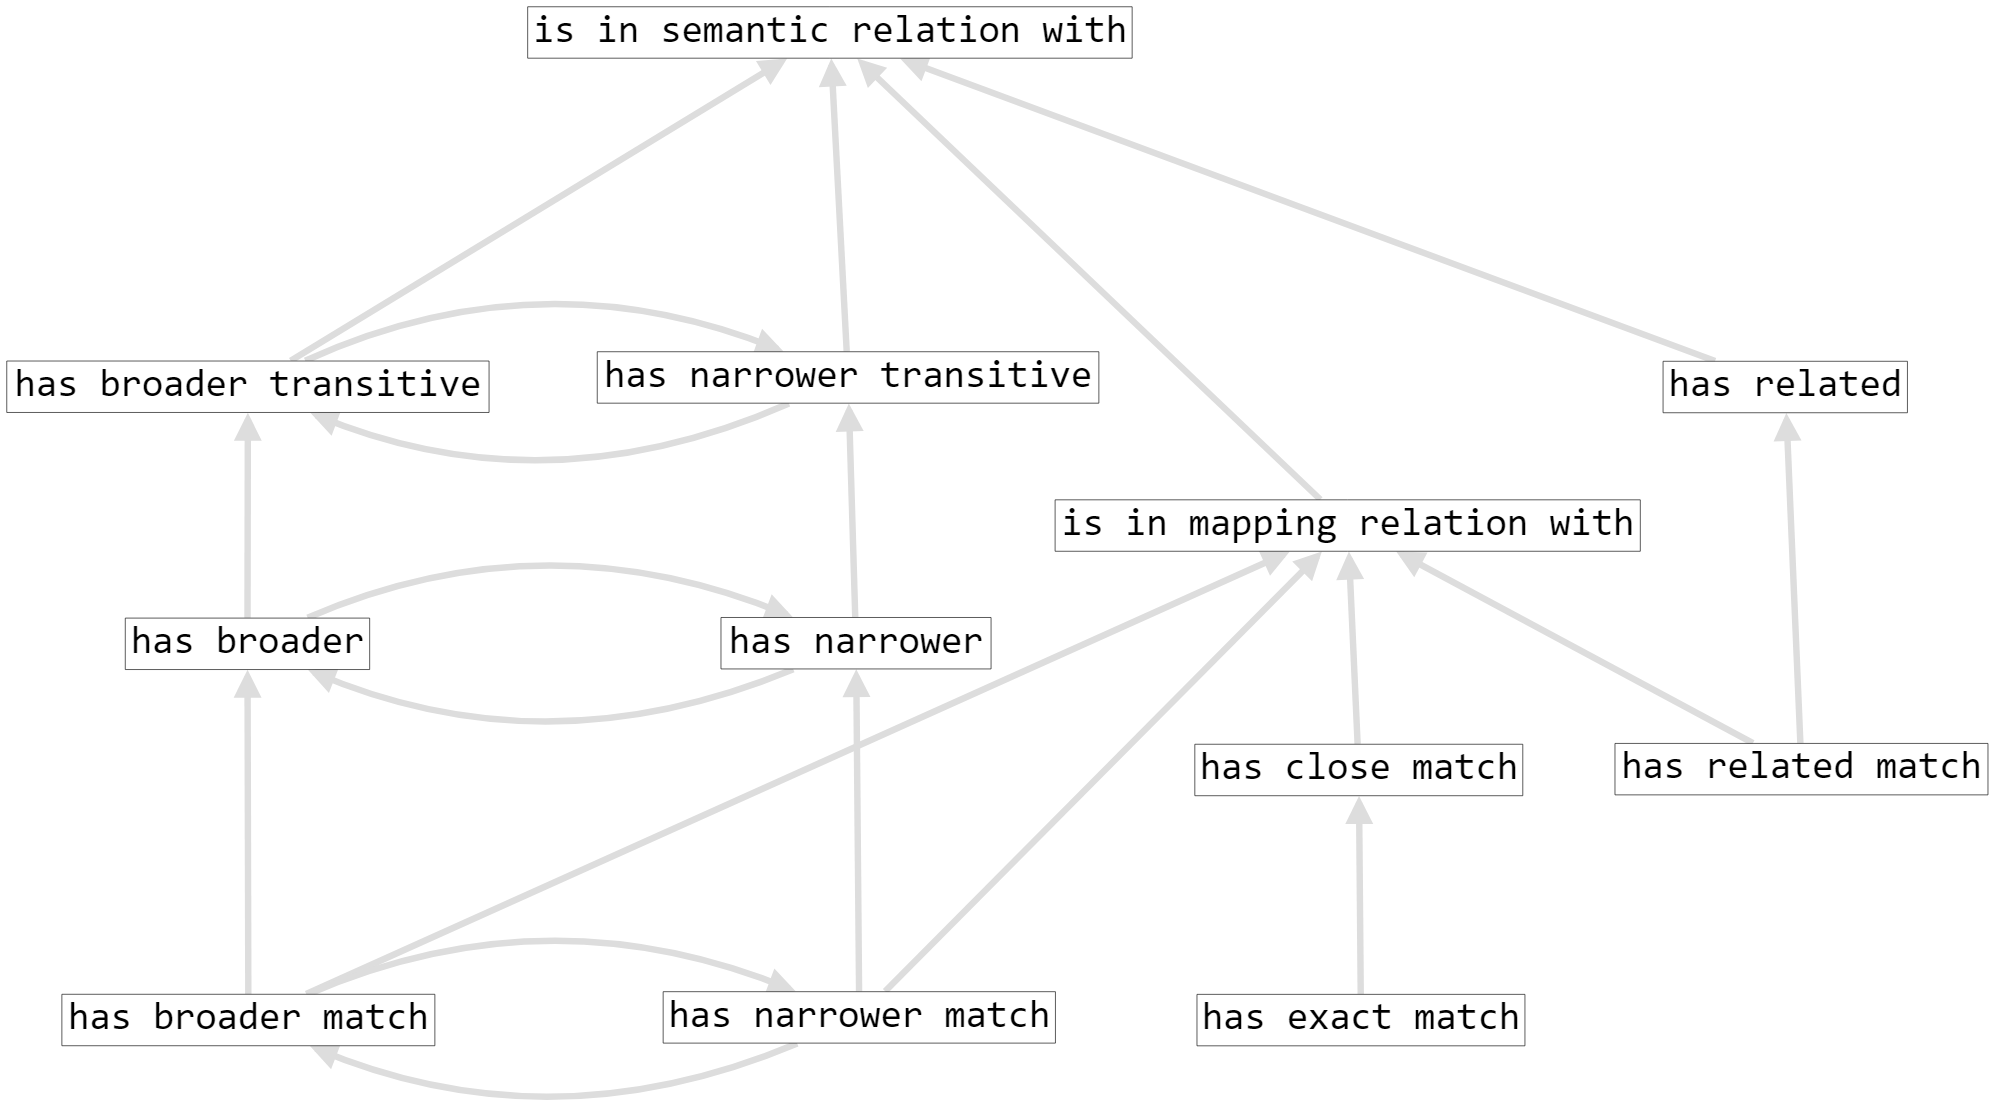
\includegraphics[width=5in]{SWWOv3/media/ch11/figure11-2i.png}
\caption{SKOS structure of Semantic Relations. Single arrows in the diagram refer to \texttt{rdfs:subPropertyOf} relationships;
double arrows are \texttt{owl:inverseOf} relationships.}
\label{fig:ch11.2}
\end{figure}





\begin{lstlisting}
agrovoc:c_4397 skos:narrower agrovoc:c_7030 .
agrovoc:c_2746 skos:broader agrovoc:c_7030 .
agrovoc:c_4163 skos:broader agrovoc:c_7030 .
agrovoc:c_6443 skos:broader agrovoc:c_7030 .
agrovoc:c_8369 skos:broader agrovoc:c_7030 .
\end{lstlisting}

Furthermore, since \texttt{skos:narrower} and \texttt{skos:broader} are subproperties of
\texttt{skos:narrowerTransitive} and \texttt{skos:broaderTransitive}, respectively, we
can infer that these things are also related with the transitive
versions of broader and narrower:

\begin{lstlisting}
agrovoc:c_4397 skos:narrowerTransitive agrovoc:c_7030 .
agrovoc:c_2746 skos:broaderTransitive agrovoc:c_7030 .
agrovoc:c_4163 skos:broaderTransitive agrovoc:c_7030 .
agrovoc:c_6443 skos:broaderTransitive agrovoc:c_7030 .
agrovoc:c_8369 skos:broaderTransitive agrovoc:c_7030 .
agrovoc:c_7030 skos:narrowerTransitive agrovoc:c_4397.
agrovoc:c_7030 skos:broaderTransitive agrovoc:c_2746 .
agrovoc:c_7030 skos:broaderTransitive agrovoc:c_4163.
agrovoc:c_7030 skos:broaderTransitive agrovoc:c_6443.
agrovoc:c_7030 skos:broaderTransitive agrovoc:c_8369.
\end{lstlisting}

and that every concept in this sample is \texttt{narrowerTransitive} than the
item at the ``top'' of the tree, \texttt{agrovoc:c}\_4397 (``Livestock''):

\begin{lstlisting}
agrovoc:c_4397 skos:narrowerTransitive agrovoc:c_7030.
agrovoc:c_4397 skos:narrowerTransitive agrovoc:c_2746.
agrovoc:c_4397 skos:narrowerTransitive agrovoc:c_4163.
agrovoc:c_4397 skos:narrowerTransitive agrovoc:c_6443.
agrovoc:c_4397 skos:narrowerTransitive agrovoc:c_7030.
\end{lstlisting}

Similar triples can be inferred (swapping subject for object, as usual)
for the inverse property,
\texttt{skos:broaderTransitive}.

In the case of \texttt{skos:related}, it is not defined as
\texttt{owl:TransitiveProperty}, so we cannot make inferences about chains of
related items. Thus, in AGROVOC, Meat is related to Meat Animals is
related to Turtles is related to Aquatic Animals is related to Mollusca
is related to Mother of Pearl, but it isn't a surprise that Meat isn't
related to Mother of Pearl. However, \texttt{skos:related} is an
\texttt{owl:SymmetricProperty} which means that since ``Mother of Pearl''
(\texttt{c\_4951}) is related to ``Decorative uses'' (\texttt{c\_2149}), that \texttt{c\_2149} is
related to \texttt{c\_4951}.

\subsection{Meaning of semantic relations}
\label{ch11.semrel}
It is no accident that there is a considerable similarity between the
definitions in SKOS of \texttt{skos:narrower} and \texttt{skos:broader} and the definition
of \texttt{rdfs:subClassOf} and superClassOf (which is not defined in the RDFS
standard). These pairs of properties are intended for modeling
hierarchies. In both cases, it is desirable that the hierarchies could
be traversed either ``upward'' or ``downward.'' In both cases,
transitivity of the relationship is important. In the case of RDF, the
transitive nature of subClassof is represented directly. SKOS uses a
more sophisticated model, in which the user of the model can decide if
they want to use a transitive notion of broader or narrower, or not.

There is one definition for subClassOf that has no corresponding
condition in SKOS. In RDFS, the type propagation rule holds.

\begin{lstlisting}
CONSTRUCT {?x rdf:type ?C}
WHERE {?x rdf:type ?B.
       ?B rdfs:subClassOf ?C . }
\end{lstlisting}

Because of this rule, there is no confusion about the interpretation of
\texttt{rdfs:subClassOf}. This rule makes it clear that C has more members (or at
least, just as many) as B; that is, C is the more encompassing of the
two classes.

Since we have no such rule in SKOS, there is the possibility for
confusion; when we say

\begin{lstlisting}
agrovoc:c_7030 skos:broader agrovoc:c_4397.
\end{lstlisting}

should we read this (in English) as ``\texttt{c\_7030} (Sheep) has broader term
\texttt{c\_4397} (Livestock),'' or should we read it as ``\texttt{c\_4397} (Livestock) is
broader than \texttt{c\_7030} (Sheep)''? There is nothing in the formal SKOS
model to tell us which is which. The relationship is expressed
informally in the annotations on \texttt{skos:broader} and \texttt{skos:narrower}; that
is, the labels ``has broader'' and ``has narrower'' respectively
indicate that the former interpretation is the intended one---Sheep has
broader term Livestock. It is important to keep this in mind when
reading the SKOS examples that follow in this book, where we will see
triples like

\begin{lstlisting}
:Sheep skos:broader :Livestock.
\end{lstlisting}

For many people, this interpretation of broader is backward from what
they expect.

If there were an inference-based definition of the semantics of
\texttt{skos:broader} (as there is, for example, for \texttt{rdfs:subClassOf}), then the
intended direction of this statement would be explicit.
There would be no need to rely on the interpretation of examples (like
this one for Sheep and
Livestock) to communicate which way the terms are intended to be used.

\subsection{SKOS and linked vocabularies}

One of the main advantages of SKOS (which it inherits from RDF) is that it allows vocabularies to be
linked. Controlled vocabularies and thesauri predate the age of the
computer. Many vocabularies were developed before there was any idea of
representing them on a computing platform, not to mention in a networked
setting. Vocabularies with this sort of heritage have been developed to
be stand-alone vocabularies, providing their own viewpoint on what words
to use to describe some domain.

In a world of computer networks, it is now common for vocabularies to
interact. A collection of content organized using one vocabulary is
presented to the same audience as a collection using another vocabulary.
The vocabularies themselves become linked information resources.

SKOS is uniquely suited for this purpose. Since SKOS is represented in
RDF, every term has a unique identifier (its URI), which can be
referenced on the Web. This makes it possible to make statements about
how a term in one vocabulary relates to a term in another.

SKOS provides a handful of matching properties exactly for this purpose:

\begin{lstlisting}
skos:exactMatch
skos:narrowMatch 
skos:broadMatch 
skos:closeMatch
\end{lstlisting}

The relationship between these properties and other SKOS properties is
shown in Figure~\ref{fig:ch11.2}. The idea of these mapping relations is that we can
express relationships between terms in different
vocabularies. We have already seen the AGROVOC concept \texttt{c\_7030}
(``Sheep''). In the United States, the National Agriculture Library
(NAL) has its own vocabulary, that includes a term \texttt{NAL:38846}
(``sheep''). What is the relationship between these two concepts? On the
face of it, we might suspect them to be the same. We can express this as

\begin{lstlisting}
NAL:38846 skos:exactMatch AGROVOC:c_7030 .
\end{lstlisting}

The property \texttt{skos:exactMatch} doesn't have any inference-based semantics.
To be more precise, there are no triples that we can infer from an
\texttt{exactMatch} that will help us to understand what it means. It does,
however, have a conventional meaning, that the two terms can be used
interchangeably across a wide range of information retrieval
applications.

While we might believe that these two terms are interchangeable, someone
else might disagree, and believe that the USDA has a more specific
notion of sheep than the United Nations does. This situation can also be
expressed in SKOS, as

\begin{lstlisting}
NAL:38846 skos:broadMatch AGROVOC:c_7030 .
\end{lstlisting}

Someone else might not be willing to make such a commitment, and instead
only believes that the two variants of the word ``sheep'' can be used
interchangeably in a few information retrieval settings. They can
express this in SKOS by saying

\begin{lstlisting}
NAL:38846 skos:closeMatch AGROVOC:c_7030 .
\end{lstlisting}

Finally, someone might want to relate a term in one vocabulary to
another, but not want to imply that they are referring to the same
thing. For instance, someone might want to record the fact that the NAL
concept for ``mutton'' (\texttt{NAL:51747}) is related to the AGROVOC notion of
``Sheep.'' There is no implication that these are the same thing, but
there is some relationship. When searching for content about mutton, it
makes sense for an information retrieval system to notify the searcher
that there could be relevant content indexed under Sheep. This can be
said in SKOS as

\begin{lstlisting}
NAL:51747 skos:relatedMatch AGROVOC:c_7030 .
\end{lstlisting}

Unlike the meanings of words like \texttt{subClassOf}, \texttt{sameAs}, \texttt{inverseOf}, etc.,
in RDFS-Plus, the meanings of the words in SKOS have much less
inference-based semantics. Their meaning is largely conventional,
referring to how they should be treated by an information retrieval
system.

But the SKOS standard is not mute about how these terms relate to one
another, and in fact SKOS uses RDFS-Plus to define those relationships.
As we have seen in Figure~\ref{fig:ch11.2}, these properties participate in an
elaborate subProperty structure. We have already seen how this structure
relates \texttt{skos:broader} to \texttt{skos:broaderTransitive}. It also relates the
matching properties to one another, and to the other SKOS properties.

In particular, we might wonder when we should use \texttt{skos:broadMatch} and
when we should just use \texttt{skos:broader}. Informally, \texttt{broadMatch} is intended
when mapping one vocabulary to another; we are stating that two terms
that were defined separately are, nevertheless, related. But will we
miss out on something, if we don't also state that they are related by
\texttt{skos:broader}?

A quick look at Figure~\ref{fig:ch11.2} can put our worries to rest. We see from the
figure that

\begin{lstlisting}
skos:broadMatch rdfs:subPropertyOf skos:broader .
\end{lstlisting}

This makes the situation clear---when we assert that a term has a
broadMatch with another term, we have also implied that it is simply
broader. The SKOS model makes it clear that we may infer that all our
matches are also related by \texttt{skos:broader}. In short, we aren't missing
out on anything by simply using broadMatch.

Similar comments apply to closeMatch and exactMatch; if we were to
assert that the NAL
notion of Sheep is an exactMatch to the AGROVOC notion of Sheep, we
could also infer that they are also a closeMatch; this is because
(again, as shown in Figure~\ref{fig:ch11.2}),

\begin{lstlisting}
skos:exactMatch rdfs:subPropertyOf skos:closeMatch .
\end{lstlisting}

In particular, if an information retrieval system were to use
\texttt{skos:closeMatch} as a means by which it determined which terms to
cross-reference, it would catch all the exact matches as well.

\section{Concept Schemes}

SKOS includes the notion of a Concept Scheme. A concept scheme is a
largely informal collection of concepts, corresponding roughly to a
particular thesaurus or knowledge organization system. While concept
schemes have little formal definition, they are useful for conveying the
intention of the publisher of one or more thesauri. Common practice for
using concept schemes is mixed. Some authorities (e.g., AGROVOC) publish
their whole vocabulary as a single concept scheme. Others (e.g., the
Library of Congress) publish each of their vocabularies using a separate
concept scheme
corresponding in part to different licensing controls on the different
vocabularies. The National
Agriculture Library uses several concept schemes, one for each
highest-level heading.

A concept scheme can be seen as a set of concepts. There are no
conditions that membership in a concept scheme be related in any way to
the semantic relations, \texttt{skos:broader}, \texttt{skos:narrower}, or \texttt{skos:related}; a
concept can be in one concept scheme while its broader and narrower
concepts are in another. Concepts are related to a concept scheme by the
properties \texttt{skos:inScheme}, \texttt{skos:hasTopConcept}, and \texttt{skos:topConceptOf}.
Concepts in a concept scheme are related to the scheme using
\texttt{skos:inScheme}. So the two
concepts \texttt{NAL:38846} (``sheep'') and \texttt{AGROVOC:c\_7030} (``Sheep'') we used
in an earlier example are in a different concept scheme, as follows:

\begin{lstlisting}
AGROVOC:c_7030 skos:inScheme <http://www.fao.org/aos/agrovoc> .
NAL:38846 skos:inScheme NAL:S .
\end{lstlisting}

We, of course, knew that these concepts were maintained by different
authorities because of their differing URIs. The explicit statement of
inclusion in a concept scheme makes this relationship explicit and
queryable with SPARQL.

A concept scheme can also have one or more distinguished concepts called
\emph{Top Concepts}. The semantic relations \texttt{skos:broader} and \texttt{skos:narrower}
define a tree structure of concepts. It is possible to find the top of
such a tree structure with a SPARQL query, but it is convenient to
indicate it with a special property. This is the purpose of
\texttt{skos:hasTopConcept} and \texttt{skos:topConceptOf}. Two triples describe the
relationship between top concepts and other members of a concept scheme:

\begin{lstlisting}
skos:topConceptOf rdfs:subPropertyOf skos:inScheme .
skos:topConceptOf owl:inverseOf skos:hasTopConcept .
\end{lstlisting}

As a result of these two triples, the top concept of a scheme must also
be in that scheme, and the properties topConceptOf and hasTopConcept are
inverses.

\subsection{Managing SKOS concept schemes}

Common practice for using these properties is varied; some vocabularies
don't use them at all (leaving membership in the concept scheme
implicit). Others use \texttt{inScheme} but make no indication of top concepts.
Among those that indicate top concepts, some use \texttt{hasTopConcept} and
others use \texttt{topConceptOf}.

All of these practices are acceptable according to the SKOS standard,
but having so many
acceptable practices, while making the job of the thesaurus writer easy,
makes it more difficult for the consumer of a vocabulary to find their way around. 
In a move toward normalizing thesaurus presentation in
SKOS, we will offer the following recommended practice for using concept
schemes:

\begin{enumerate}
\item Align concept schemes to your own governance practice. In particular,
use one concept scheme per vocabulary that is controlled by a single
work process.

\item Propagate membership in concept schemes across \texttt{skos:broader} and
\texttt{skos:narrower}. That
is, the inference given by the following SPARQL CONSTRUCT should be
valid:

\begin{lstlisting}
CONSTRUCT {?c skos:inScheme ?S }
WHERE {?a skos:inScheme ?S .
       ?a skos:broader ?c .}
\end{lstlisting}

A similar rule holds for \texttt{skos:narrower}.

\item Use \texttt{skos:broadMatch} (resp. \texttt{skos:narrowMatch}, \texttt{skos:exactMatch},
\texttt{skos:closeMatch}) only to map concepts that are in different concept
schemes.

\item Indicate the top of all \texttt{skos:broader} trees with \texttt{skos:hasTopConcept}.
Do not indicate any concepts internal to the tree as top concepts.

\item Keep the number of top concepts in any single concept scheme small
(i.e., fewer than a half dozen)

\end{enumerate}

These guidelines are intended to provide some coherence to SKOS
presentation, but are not normative in any way. They are motivated by
experiences made while reading vocabularies prepared by a variety of
authorities. While there may be good reasons to break any of these
rules, keeping to them ensures that thesaurus presentations are not
surprising (e.g., keeping concepts in a single scheme together in the
same broader/narrower tree), and that it is easy for someone searching a
vocabulary to know where to start (by indicating the top concept). Some
of them are just common sense (e.g., not indicating internal nodes as
``top'' concepts), while others are somewhat arbitrary (e.g., why
stipulate \texttt{hasTopConcept} instead of \texttt{topConceptOf}?).

The existence of concept schemes provides an example of the motivation
for having the property
\texttt{skos:exactMatch}, even in light of the extant and very similar property
\texttt{owl:sameAs}. The semantics of \texttt{owl:sameAs} state that any two resources
that are \texttt{sameAs} one another are interchangeable in every statement.
This means that if two concepts were \texttt{sameAs} one another, then they would
necessarily be in the same concept scheme. Since concept schemes reflect
authority and work process, this is clearly not appropriate. The
property \texttt{exactMatch} makes much less commitment to interchangeability of
concepts, indicating only that one concept acts like the other in
information retrieval settings.

\section{SKOS Integrity}

While many things in SKOS are not formally defined by inferences, SKOS does
include a number of integrity conditions that can be applied to any SKOS
model to verify that it conforms to the standard. These conditions are
normative, in that a model that violates them cannot be said to be
conformant to the standard. There are 46 such conditions on the core
SKOS ontology. We will not cover all of them in this book, but by
examining a few of them, we hope to convey the basic idea of how SKOS is
intended to be used.

Many of the constraints can be (and are) expressed in RDFS. In fact, all
of the relationships shown in Figure~\ref{fig:ch11.2} are part of the SKOS
constraints, along with domain/range information such as:

\begin{lstlisting}
skos:inScheme rdfs:range skos:ConceptScheme .
skos:semanticRelation rdfs:domain skos:Concept .
skos:semanticRelation rdfs:range skos:Concept .
\end{lstlisting}

That is, if something is in a scheme, then the thing it is in a
\texttt{skos:ConceptScheme}. Any two things related by any semantic relation
(that includes broader, narrower, related, and all the matching
relations) are both members of the class \texttt{skos:Concept}.

Other constraints are most easily represented in SPARQL. We can use an
ASK query to specify Boolean conditions in SPARQL; thus we can specify a
condition that evaluates as true if there is a violation of the
constraint. For instance, one constraint says that a resource has no
more than one value of \texttt{skos:prefLabel} per language tag. This can be
expressed in SPARQL as

\begin{lstlisting}
ASK
WHERE {?c skos:prefLabel ?l1 .
       ?c skos:prefLabel ?l2 .
       FILTER (lang (?l1) = lang (?l2))
       FILTER (?l1 != ?l2)
}
\end{lstlisting}

This query uses the function lang(?x) that returns the language tag for
a string (``en'' for English, ``fr'' for French, and so on). If the
language tag matches for two different strings (i.e., they don't match),
then we have a violation of the constraint.

Certain properties are constrained to be disjoint, e.g., \texttt{skos:related}
and \texttt{skos:broaderTransitive}. That is, if two concepts are related, one
cannot have the other as a broader term. This can be expressed in SPARQL
as

\begin{lstlisting}
ASK
WHERE {?a skos:related ?b .
       ?a skos:broader* ?b }
\end{lstlisting}

That is, it is a violation if \texttt{?a} and \texttt{?b} are related, and one is broader
(transitive) than the other.

In general, the integrity constraints in SKOS guarantee that a
vocabulary is orderly, in a manner conducive to its use (and re-use) in
information retrieval settings. It wouldn't do for a single concept to
have two preferred labels in the same language, and once you know that
one concept is broader than another, there is no need to shortcut this
by making them related concepts as well.

\section{SKOS in Action}

SKOS is a great example of what we have in mind when we call something
``a model on the Semantic Web''; it models particular standards for how
to represent thesauri in a Web-oriented way that encourages linking and
reuse. We have seen what this model says about terms and concepts in a
thesaurus and how they can relate to one another. But how is SKOS itself
being used? What do we gain by representing a thesaurus in SKOS?

Utilization of the SKOS standard has grown dramatically since the W3C
made it a Recommendation (second version in 2008). In addition to
AGROVOC and the US National Agriculture library, many large-scale
thesauri have been published in SKOS, including the Library of Congress
Subject Headings, the West Key Numbering System, and EUROVOC, as well as
a multitude of smaller scale vocabularies.
What has driven the popularity of SKOS? There are a number of factors
involved.

First is its simplicity. The initial ``\textbf{S}'' in SKOS stands for
``Simple,'' and the committee succeeded in large part in making it
simple. This means that vocabularies represented in just about any other
vocabulary system can be translated to SKOS without a lot of effort. The
basic SKOS relationships
(broader, narrower, related) and classes (Concept, ConceptScheme) do a
good job of capturing what is essential in vocabularies.

Second is the ease with which a vocabulary can be transformed from other
systems into SKOS. For the most part, if it is possible to query an
existing vocabulary for broader, narrower, and related terms, then the
vocabulary can be converted directly into SKOS. Simply record the
outcome of that query as a triple:

\begin{lstlisting}
?narrow skos:broader ?broad .
\end{lstlisting}

The simplicity of this process has enabled a cottage industry of SKOS
conversions. It is not uncommon to see vocabularies that have been
traditionally presented in spreadsheets, XML, databases and other
storage formats published in SKOS.  In Chapter~\ref{ch14} we'll see how FIBO, the Financial Industry Business Ontology, is published in both OWL and SKOS using this method. 

A closely related factor is that until SKOS, there was no \emph{de jure}
standard way to represent a vocabulary in digital form. This is a
surprising state of affairs, brought about in part by the dominance of
many proprietary digital vocabulary forms, and the failure of
non-proprietary forms to gain the stamp of approval of a major standards
body. While there are many thesaurus standards supported by groups like
ISO and NISO, these standards did not include normative recommendations
for how to store a thesaurus in digital form.

The final factor is more subtle. Translation of a vocabulary into SKOS
involves selecting a globally
unique identifier for each concept. In practice, this is not a difficult
thing to do (most thesauri already have some locally unique identifier
anyway; e.g., the West Key Numbering System has its key numbers; the
Library of Congress Subject Headings have their own identifiers). But
translation into SKOS turns these locally unique identifiers into
globally unique identifiers. This provides a great advantage when
relating vocabularies to one another. As organizations merge and as
information is published on a worldwide scale, it becomes more and more
necessary to be able to link one vocabulary to another. This Web-enabled
aspect of vocabulary management is something that older thesaurus
standards (developed pre-Web) were not designed to support.

The case of AGROVOC and the NAL vocabulary illustrates this advantage.
Shortly after the introduction of SKOS, the United Nations pursued a
project to map these two thesauri together. The project needed a
representation that would allow for terms from the two sources to be
distinguished from one another. For example, the AGROVOC word for
``Groundwater'' and the NAL word for ``groundwater'' must be managed
separately, but it also must be possible to represent the relationship
between them. The point of the project was to compare and manage
proposed relationships between them---is the AGROVOC notion of
``Groundwater'' the same as the NAL notion of ``groundwater''? Or is it
broader? Or narrower? Or just closely related? Whatever conclusion one
proposes, it is necessary to be able to talk about the AGROVOC term and
the NAL term in the same statement. The translation of terms into URIs
makes it possible to relate these things with a single triple, e.g.,

\begin{lstlisting}
NAL:11571 skos:broadMatch AGROVOC:c_3391 .
\end{lstlisting}

\section{SUMMARY}

SKOS demonstrates how a fairly simple set of modeling constructs can be
used to create extensible, distributed information networks. SKOS takes
advantage of the distributed nature of RDF to allow
extension to a network of information to be distributed across the web.
It relies on the inferencing structure of RDFS-Plus to add completeness
to their information structure.

SKOS vocabularies provide a cornerstone for linking information on the
web. In order for two information sources to integrate, they have to
have some common ground. Controlled vocabularies are the best candidate
for such common ground. Publishing vocabularies in SKOS allows the
concepts they define to be referenced on a global scale.

Controlled vocabularies are everywhere---not just in high-profile places
like the United Nations or
the Library of Congress. Anything that has a standard, official name can
be used in a controlled vocabulary. Names of universities, stock symbols
of companies, place names, names of months, all of these things are
controlled vocabularies. Many of them have been published in SKOS, and
many more are under way.

\subsection{Fundamental concepts}

The following fundamental concepts were introduced in this chapter.

Controlled Vocabulary---A set of terms providing common reference for
linked information systems.

SKOS---Namespace for a system of representation for information
management. SKOS stands for

``Simple Knowledge Organization System.''

AGROVOC---The United Nations agriculture vocabulary, see
\url{http://aims.fao.org/website/} AGROVOC-Thesaurus.

NAL---the National Agriculture Library, see
\href{http://agclass.nal.usda.gov/}{http://agclass.nal.usda.gov/.}
